\documentclass[colorlinks=true,pdfstartview=FitV,linkcolor=blue,
            citecolor=red,urlcolor=magenta]{ligodoc}

\usepackage{graphicx}
\usepackage{amssymb}
\usepackage{amsmath}
\usepackage{longtable}
\usepackage{rotating}
\usepackage[usenames,dvipsnames]{color}
\usepackage{fancyhdr}
\usepackage{hyperref}
\usepackage{array}
\usepackage{subcaption}
\usepackage[dvipsnames]{xcolor}
\usepackage[title]{appendix}

\ligodccnumber{T}{11}{T2200282}{}{v0}% \ligodistribution{AIC, ISC}

\title{Methods of Improving Optical Contacting

Second Interim Report}

\author{Jennifer Hritz}

\begin{document}

%##############
%For draft only
\begin{center}
\LARGE
{\color{red} DRAFT 2}
\end{center}
%##############

\begin{center}
\textbf{Abstract}
\end{center}

This project will attempt to improve optical contacting between silicon objects. There will be a focus on the use of heat and pressure to increase the strength of the bond. The eventual goal is to make optical contacting strong enough to be a viable method for conjoining pieces of high precision equipment in space, specifically for the LIGO Voyager.

\section{Background}
Optical contacting is the phenomenon of bonding very flat, highly polished surfaces together using Van der Waals dispersion forces instead of adhesives. Van der Waals dispersion forces are weak at large distances, but by bringing many atoms and molecules very close together, it makes for an incredibly strong bond. The cleaner and flatter the surface, the closer the atoms and molecules, and therefore the stronger the bonds. To avoid contamination and deviations from flatness, polishing and cleaning are important steps before optically contacting two plates \cite{Wright}.

When performed properly, the bond between the two surfaces is strong enough to effectively merge the two objects into one. The applied force is concentrated at the edge, so while pulling apart the two plates is difficult, the bond can be easily broken by wedging the plates apart at an edge or corner \cite{Rayleigh}. The only other way to destroy this adhesion is through thermal stress, where unequal heating causes thermal expansion to break the closeness of the surfaces \cite{Ferme}. Hence, two ways to test the efficacy of the bond can be tested by determining the tensile strength and measuring heat flow \cite{Wright, Zawada}.

Adding heat and applying pressure have been shown to improve the quality of the bond \cite{Zawada}. Optical contacting could theoretically occur between any two surfaces, but it is typically performed with silicon, or silicon-containing molecules due to its weight and thermal properties.

\section{Motivation}
\changestart[blue]
Optical contacting has big uses in space because it produces strong, light bonds without adhesives. When two objects are bonded with adhesives, the bond risks failing due to the adhesive having different chemical and thermal properties. From the bonded objects. Silicon’s small thermal expansion coefficient makes it particularly useful for high sensitivity probes \cite{Wright} including gravitational wave detectors such as LISA and the LIGO Voyager.

However, before optical contacting can be applied in space, it needs to be studied further. The aim of my research is to explore methods of optimizing optical contacting to produce a consistently strong bond. This includes refining previous work which indicated that heat and pressure were instrumental in producing good bonds. If I can produce sufficiently strong bonds, I will proceed to working on their application in the LIGO Voyager. This means I also need to attempt to the answer the question of what is a sufficiently strong bond.

\section{Approach}
In a sterile environment, I will optically contact first glass slides and later silicon wafers. This involves thoroughly cleaning the surfaces, placing one clean surface over the other at a right angle, and gently pressing to form the bond. I will add weight on top of the sample and apply heat using a hot plate during the bonding process to produce a higher quality bond.

Once the bond has been made, I assess its quality by finding the 1) shear and/or tensile strength 2) thickness of the gap 3) mechanical quality of the bonded objected.

Finding the shear strength involves measuring the amount of parallel force it takes to make the bond slip. This means pushing or pulling on one half of the sample in a controlled manner. In addition to or in replacement of---if finding the shear strength is too difficult---this experiment, I will also find the tensile strength of the bond. This is carried out by carefully wedging a razor blade between the seam of the bond and measuring the gap from the tip of the razor to the edge of the unbroken bond. Straightforwardly, the stronger the shear or tensile strength, the stronger the bond.

Finding the thickness of the gap requires ellipsometry, which is the process of extracting information using the change in polarization when a polarized laser is reflected by a thin film. The wider the gap, the weaker the bond.

Determining the mechanical quality of the bonded object shows bond quality because if the mechanical quality is close to that of solid silicon, the two objects have effectively become one. This will be tested by constructing a tuning fork---an acoustic resonator tuned to a specific note from which pianos are tuned---using optical contacting and testing its resonance. The optically contacted tuning fork will be constructed of two silicon single-crystal silicon wafers attached to the end of another silicon single-crystal silicon wafer in the shape of a tuning fork. The tuning fork is then placed in a vacuum, resonated with electricity, and the vibrations are recorded by a laser.

\section{Work completed}

I started by designing the experiments to test the bond quality. These are still in varying degrees of drafting stages and can be found in Appendix \ref{appendix:bond_quality_experiment_drafts}. I also designed the setup for applying heat and pressure to the sample, which can be found in Appendix \ref{appendix:pressure_heating_setup}.

\subsection{Hot plate}

I started by first determining the heating properties of the hot plate using a thermocouple. Since the bonded samples will need to be heated evenly at a precise temperature, I measured the maximum temperature at each dial setting and the temperature at different locations on the hot plate, as seen in Figure \ref{fig:hotplate_heat_test_setup}.

\begin{figure}[htbp]
\begin{center}
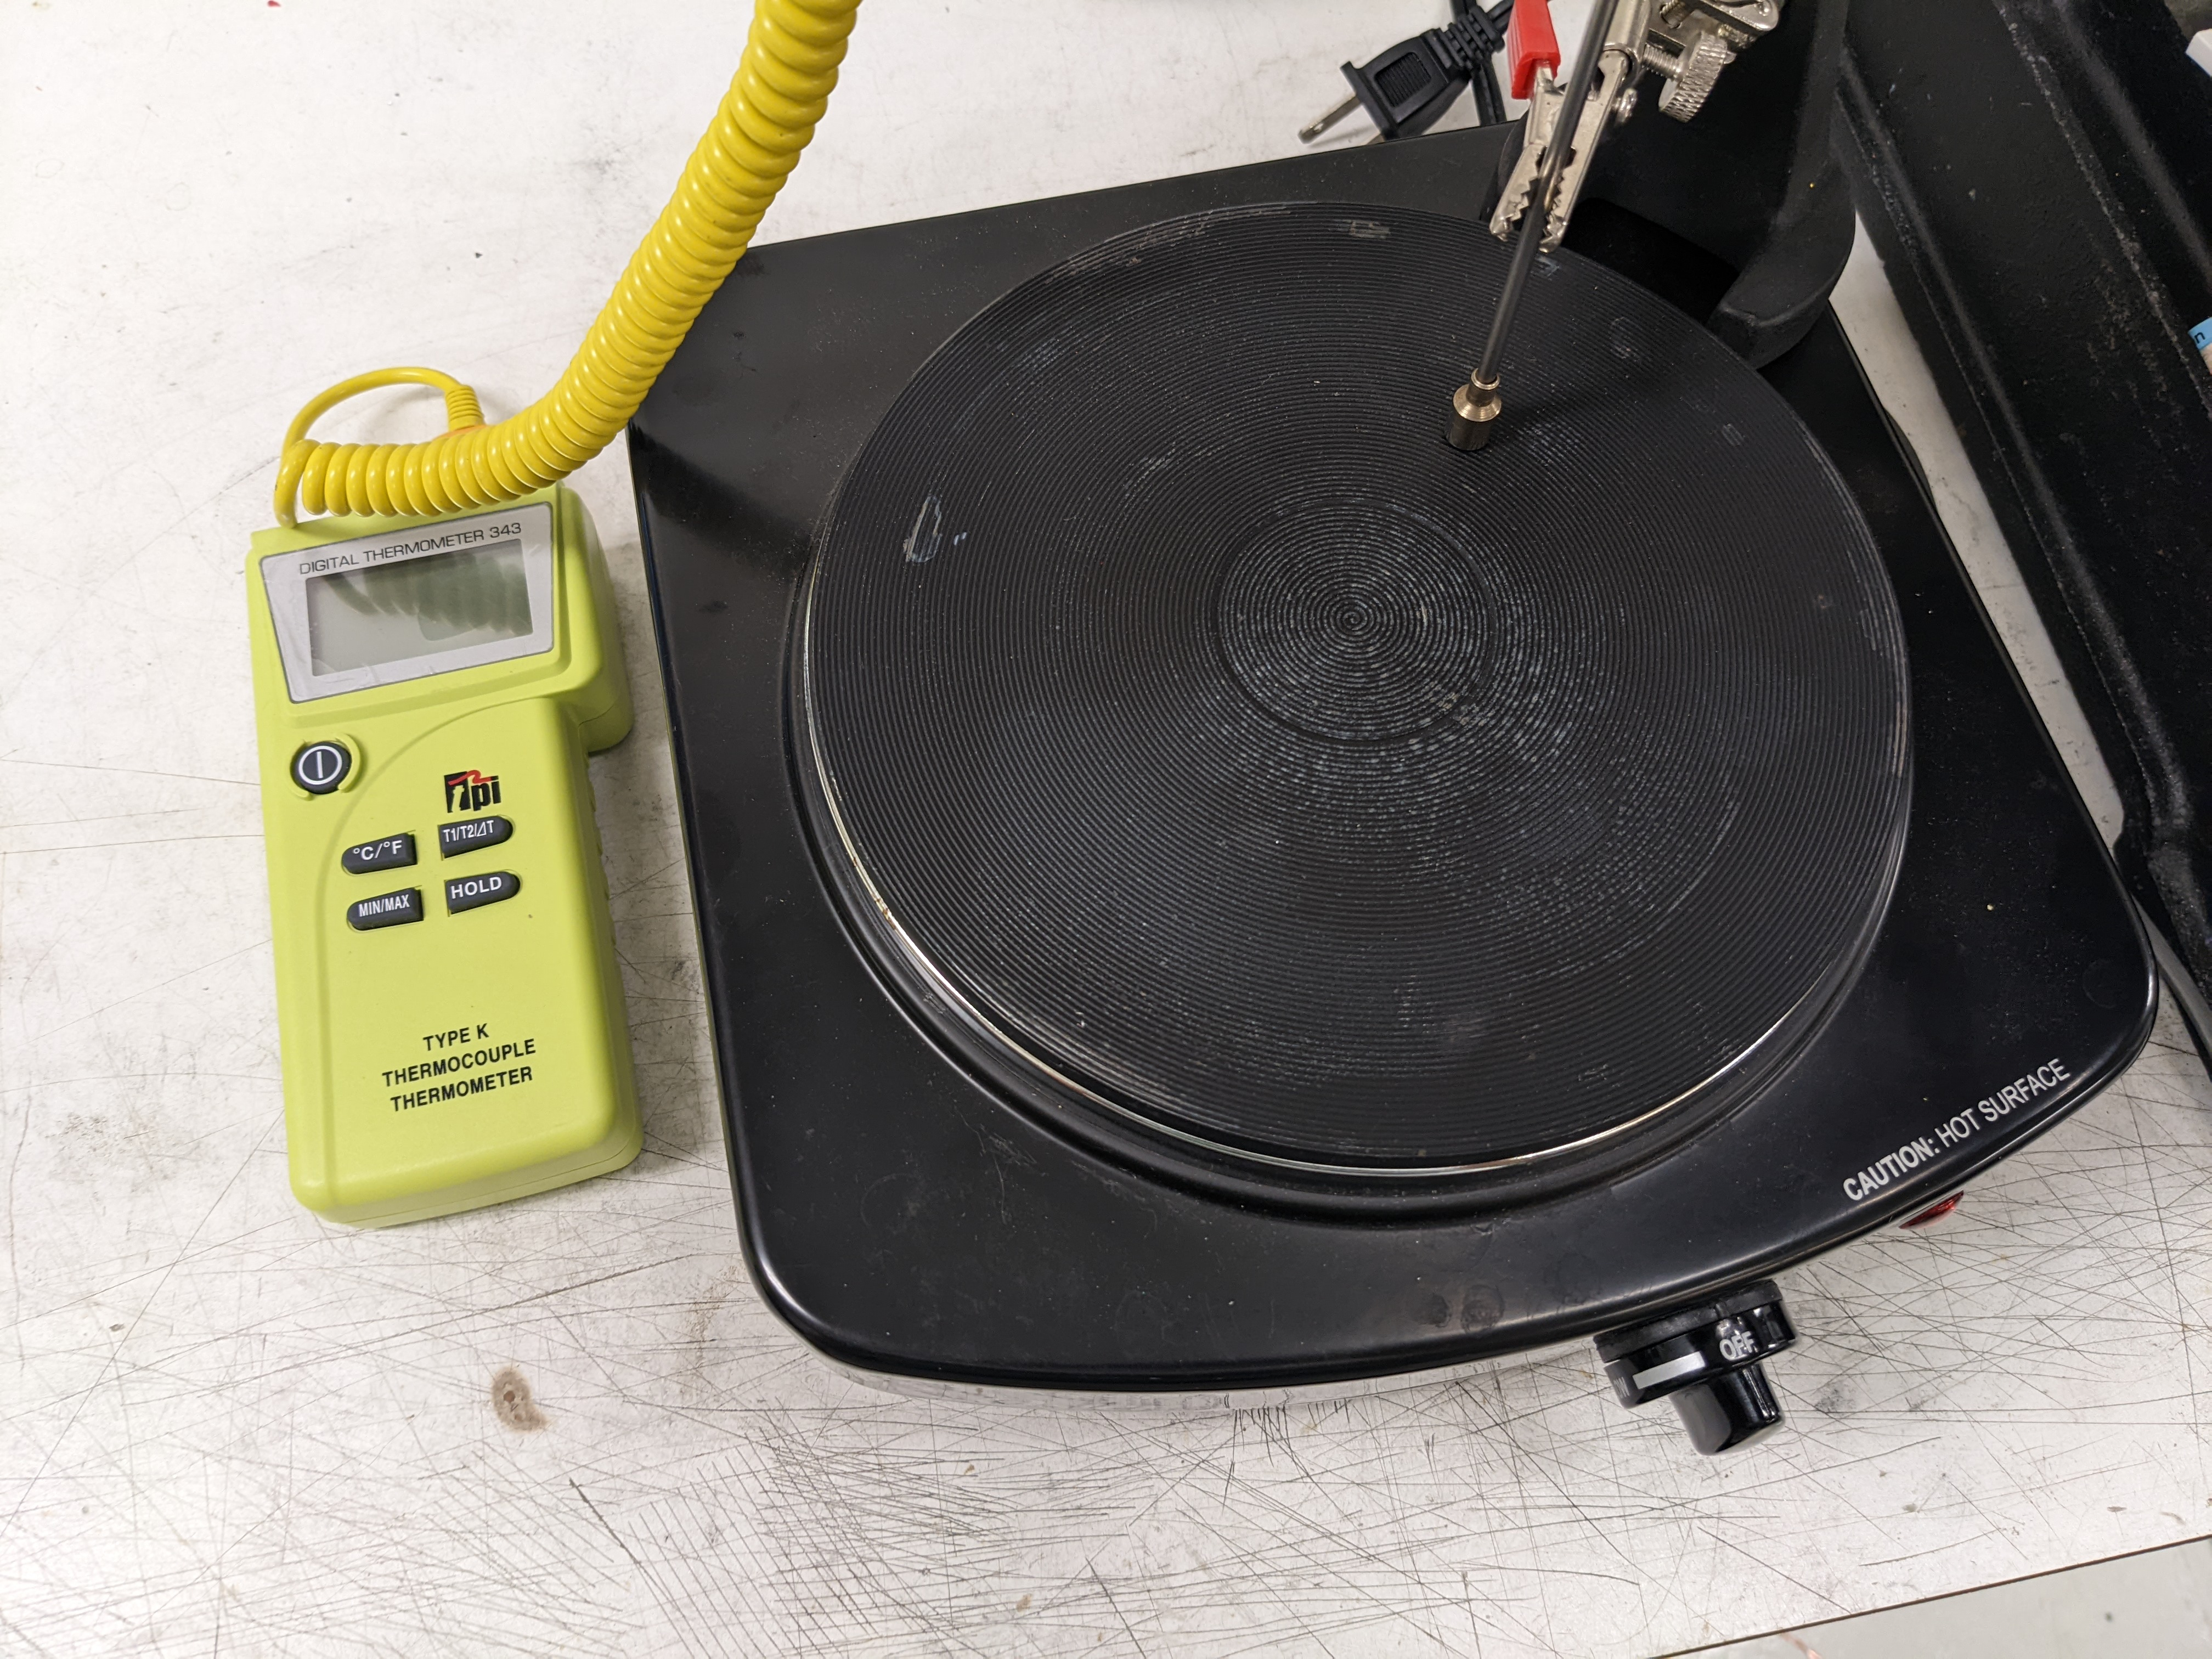
\includegraphics[width=6in]{graphics/hotplate_heat_test_setup_PXL_20220708_230032062.jpg}
\caption{The Type K thermocouple was attached to the Digital Thermometer 343, and the measuring tip of the thermocouple was mounted parallel against the Oster hot plate. Per the thermometer manual, the tip must be held in place for at least 30 seconds to get an accurate reading.}
\label{fig:hotplate_heat_test_setup}
\end{center}
\end{figure}

To measure the maximum temperature at each setting, I turned the dial and waited until the temperature of the thermometer stayed constant for over 1 minute. I then recorded the exact temperature and the rough time it took to stabilize (Figure \ref{fig:hotplate_heat_test_setup}). Once the data was collected, I turned the dial to the next setting, performing this for the low, medium, and high settings.

\begin{figure}[htbp]
\begin{center}
  \begin{tabular}{ | l | c | c | c | c | c | }
    \hline
    Setting & Off & Low & Medium & High & Off (Again) \\ \hline
    Max. temp. (°C) & 26.2 & 51.3 & 185.0 & 263.5 &N/A \\ \hline
    Time to temp. (min)  & N/A & 5.5 & 7.0 & 6.0 & $\sim$ 3 hours \\
    \hline
  \end{tabular}
\end{center}
\caption{The results of finding the maximum temperature at each hotplate knob setting. Note that "Time to temp." is the time from when the dial was switch up to when the temperature stabilized. The times are meant to only be rough estimates since I was multitasking during the experiment and not watching the plate the entire time. "Off (Again)" is the rough amount of time it took for the plate to completely cool down.}
\label{fig:hotplate_max_heat_data}
\end{figure}

Once the temperature at the high setting stabilized, I moved the thermocouple to different parts of the hot plate, being careful to keep the measuring tip parallel and to hold it steady for over 30 seconds. As seen in \ref{fig:even_heating_test_results}, the top right corner is slightly cooler and the hot plate is the hottest in a ring at about half the radius, likely where the heating coil sets.

\begin{figure}[htbp]
\begin{center}
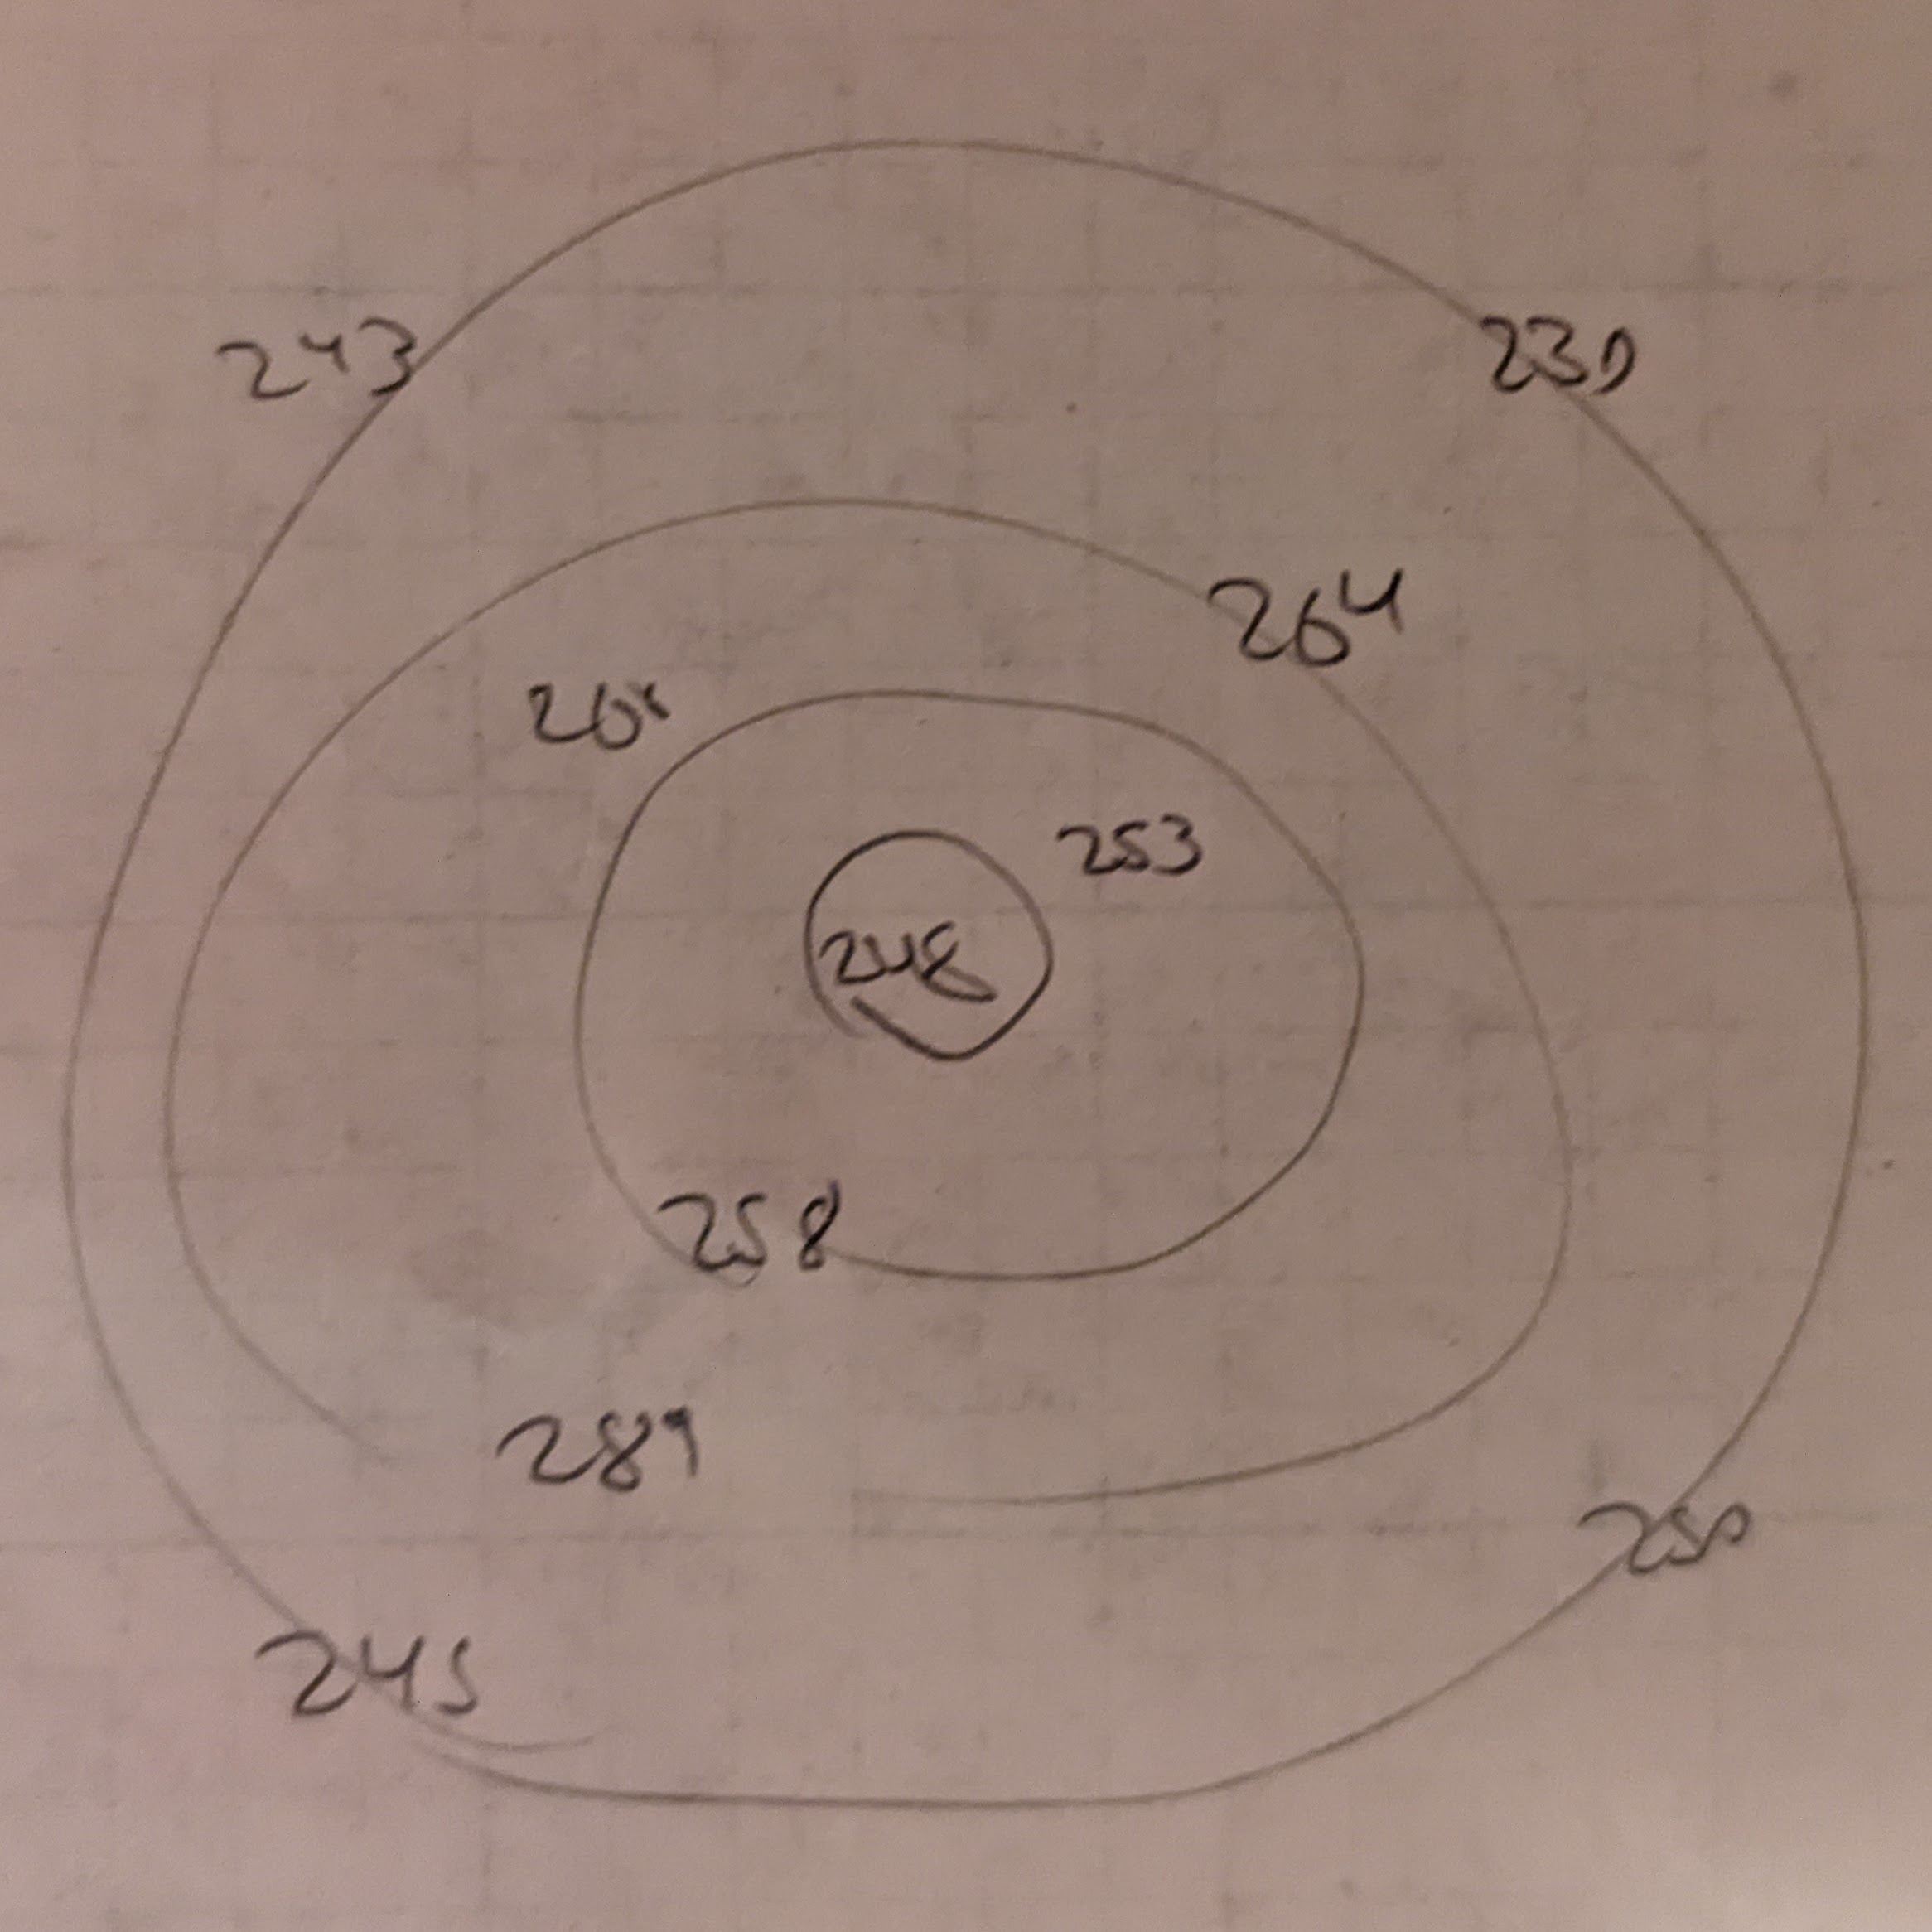
\includegraphics[width=6in]{graphics/even_heating_test_results_PXL_20220729_050013935.jpg}
\caption{The temperature (°C) at different points on the hot plate. The bottom of the circle is the side of the hot plate with the nob. It was a coincidence that the  thermocouple was set up in the cool corner during the maximum temperature test.}
\label{fig:even_heating_test_results}
\end{center}
\end{figure}

This was meant to be a rough baseline test. Once I find a way to control the temperature beyond the three settings, I will need to repeat it with a newer, more accurate multimeter.

\subsection{Bonding}

Before working with delicate silicon wafers, I started with attempting to bond 25 mm x 75 mm x 1.1 mm borosilicate glass microscope slides manufactured by Globe. I tried a variety of methods to get a feel for what worked and what did not.

I began by gently cleaning the slides with Kimwipes then carefully laying one slide on top of the other. When the top slide was lifted up, the bottom slide would hang on for at most a couple seconds before gravity overcame the bond (Figure \ref{fig:kimwipe_bond}). Pressure, with my fingers or a large brass rectangle and heat, on any of the settings, as well as the two combined did not improve the bond.

\begin{figure*}[t!]
    \centering
    \begin{subfigure}[t]{0.3\textwidth}
        \centering
        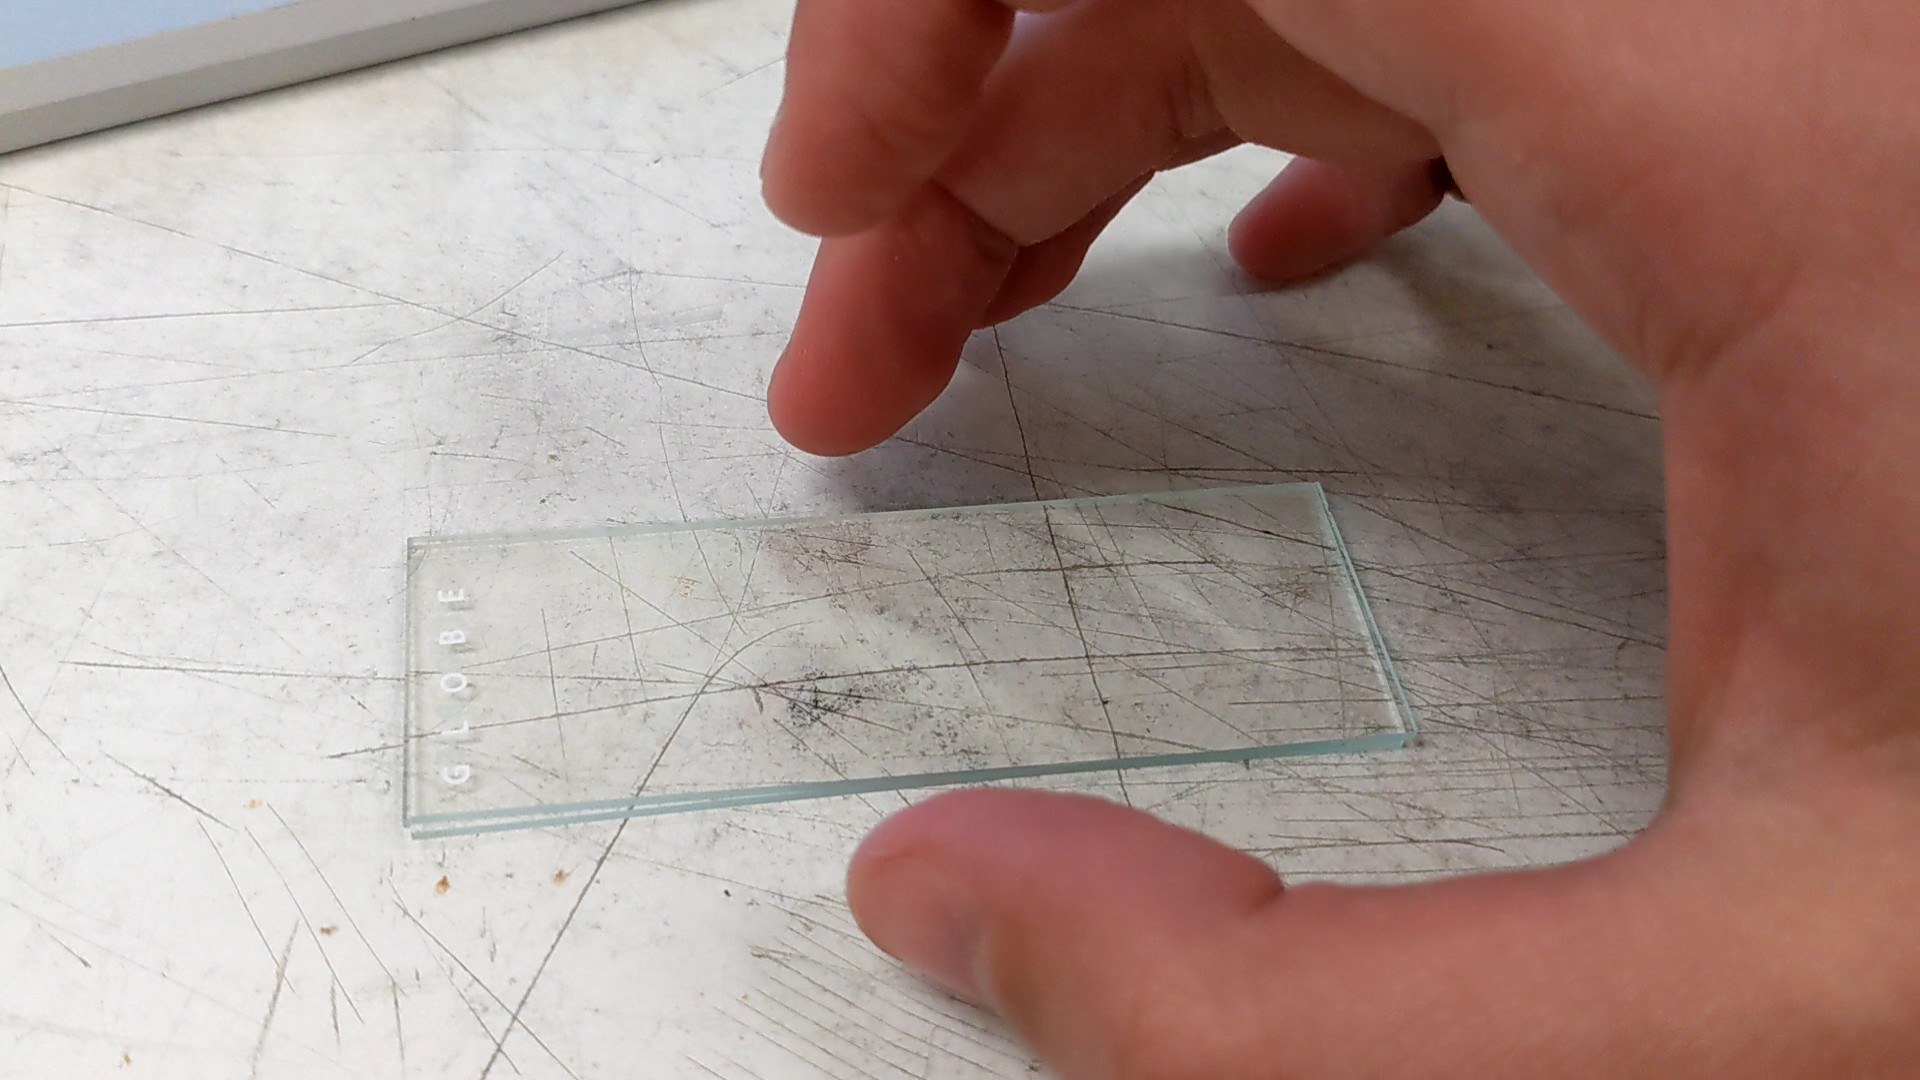
\includegraphics[width=1.75in]{graphics/kimwipe_before_PXL_20220712_003150428_exported_33.jpg}
        \caption{After bonding attempt.}
    \end{subfigure}%
    ~ 
    \begin{subfigure}[t]{0.3\textwidth}
        \centering
        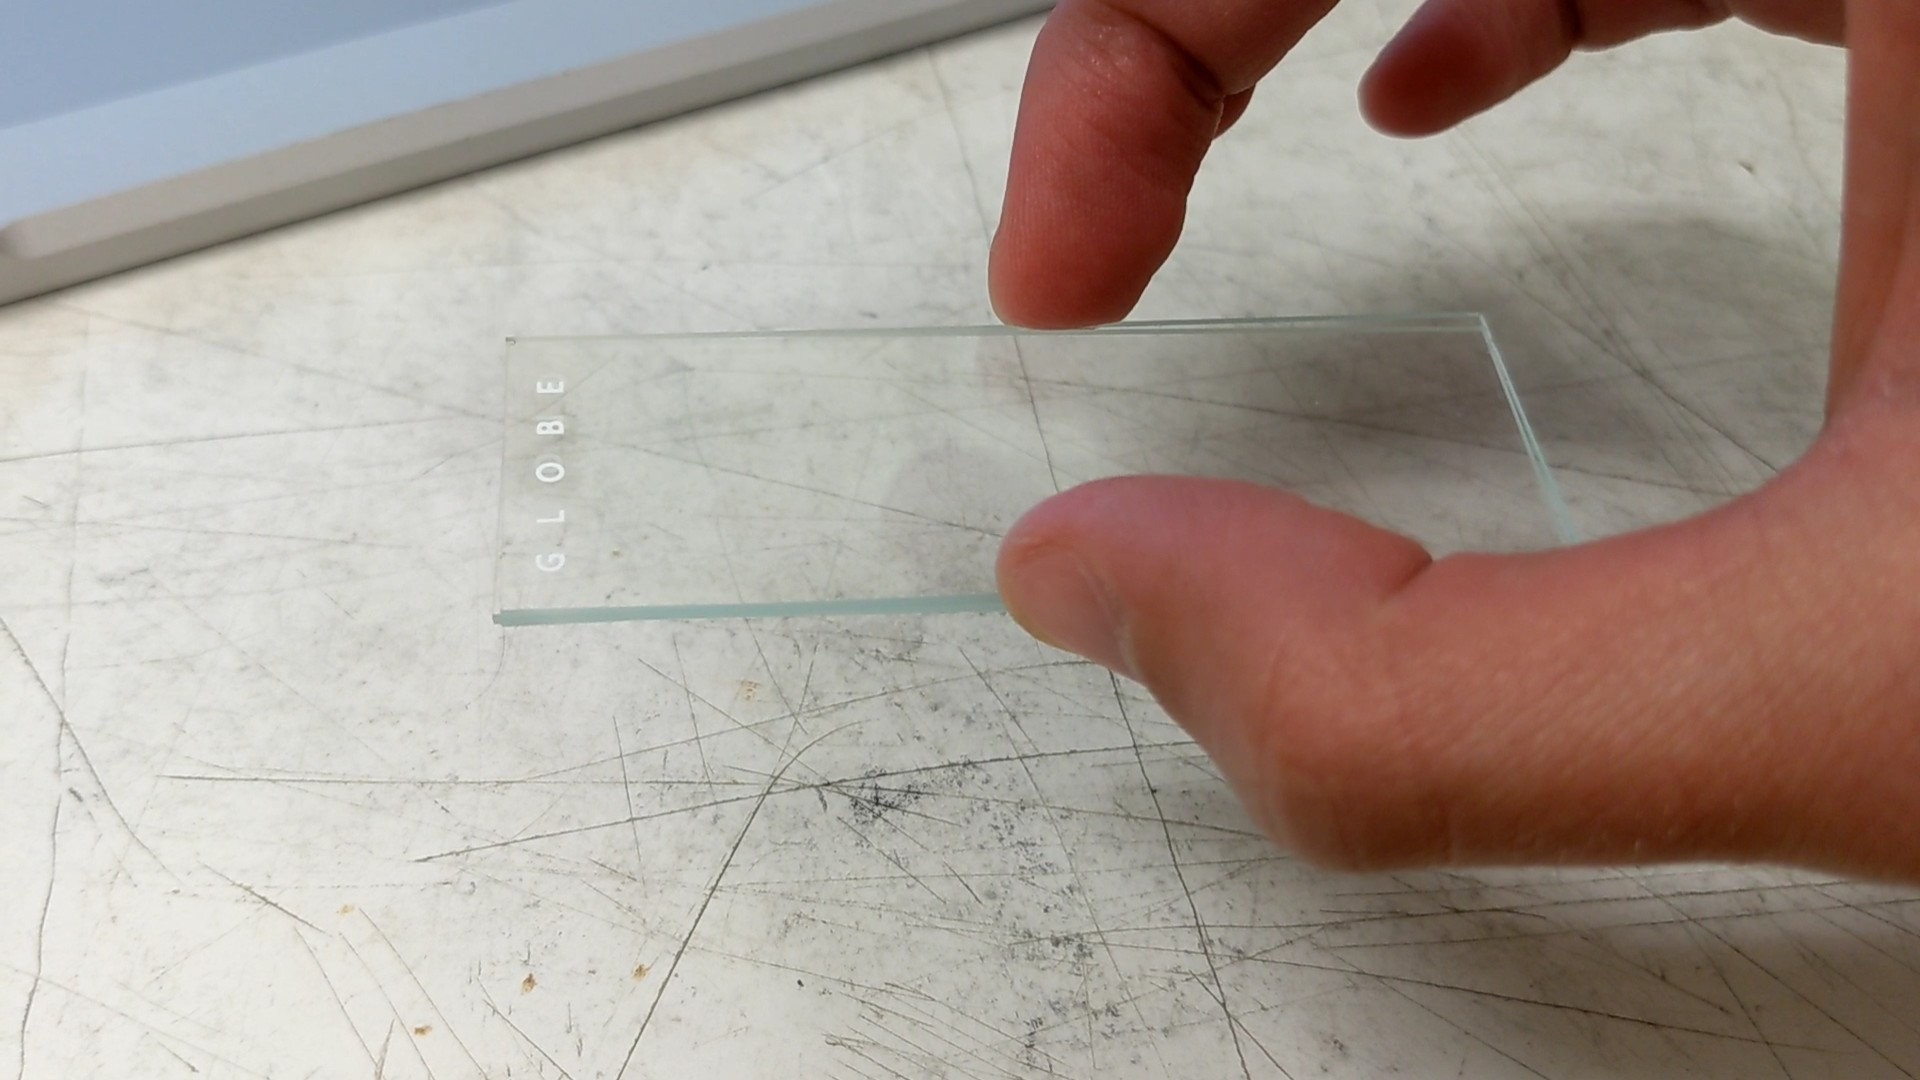
\includegraphics[width=1.75in]{graphics/kimwipe_during_PXL_20220712_003150428_exported_3069.jpg}
        \caption{The bond briefly holding.}
    \end{subfigure}%
    ~ 
    \begin{subfigure}[t]{0.3\textwidth}
        \centering
        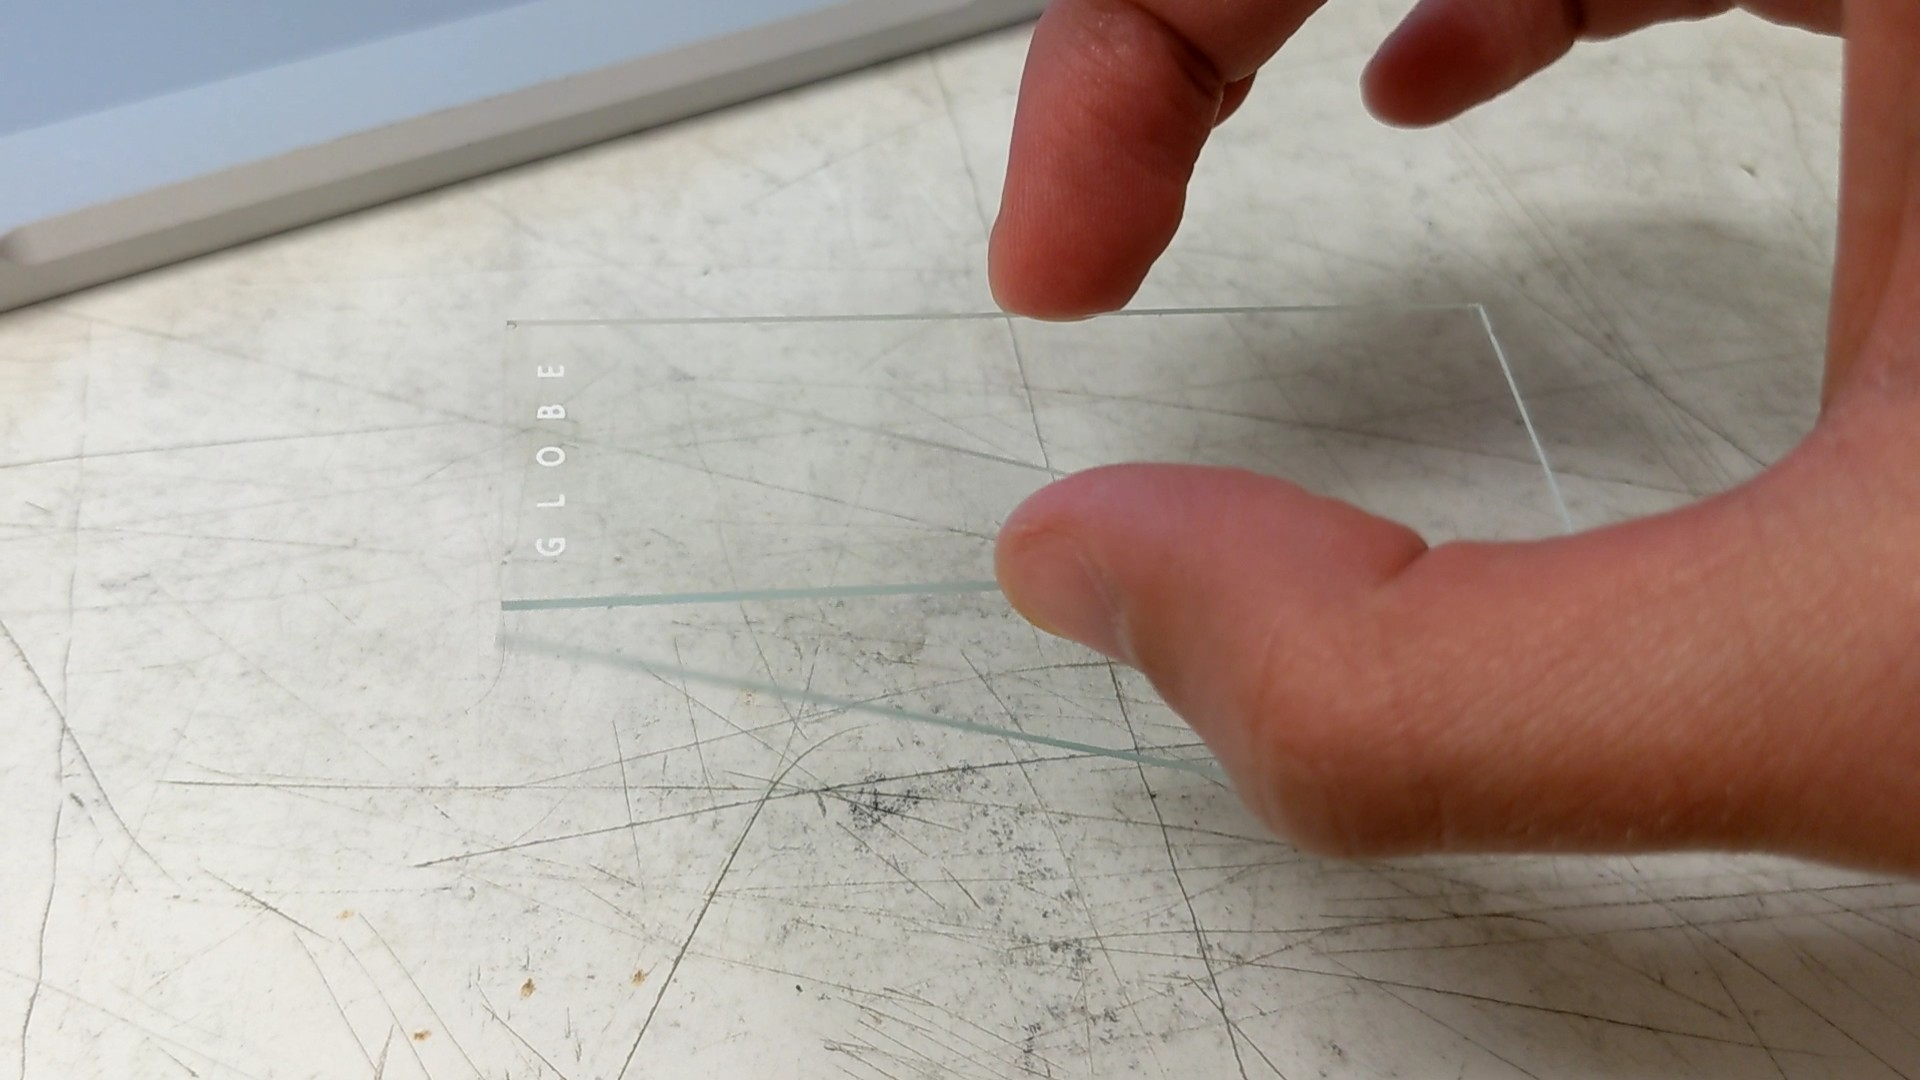
\includegraphics[width=1.75in]{graphics/kimwipe_after_PXL_20220712_003150428_exported_3069.jpg}
        \caption{Failure of the bond.}
    \end{subfigure}%
    \caption{These demonstrate the failure of a bonding attempt using just Kimwipes to clean the glass}
    \label{fig:kimwipe_bond}
\end{figure*}

While drying two slides after washing them to remove my fingerprints, I discovered that sticking the two slightly wet slides together made a bond strong enough that it took all the strength in my fingers to make them slide slightly apart. This was my first successful bond. If it is difficult or outright impossible for me to separate the slides with my fingers, I consider the slides to now be a bonded sample. Since, so far, all of my samples instantly come apart when I put a razor blade between them, my only test of strength is "can I pull/slide it apart with my fingers?"

Having found a trick to performing the bond, I began qualitatively experimenting with different liquids and bonding methods. To prepare a sample, I would drop the liquid on one slide then squish the other slide on top of it, ensuring that the liquid filled the entire gap. As the liquid left the gap or evaporated, the bond would form. I tested this method with water, isopropanol, or methanol. They all were successful in producing bonds, but qualitatively, methanol seemed to produce the best bond. Applying pressure  without heat (Figure \ref{fig:squished_sample} did not appear to improve the bond. Leaving the samples overnight to let the liquid completely exit the gap slightly improved the bond strength.

\begin{figure}[htbp]
\begin{center}
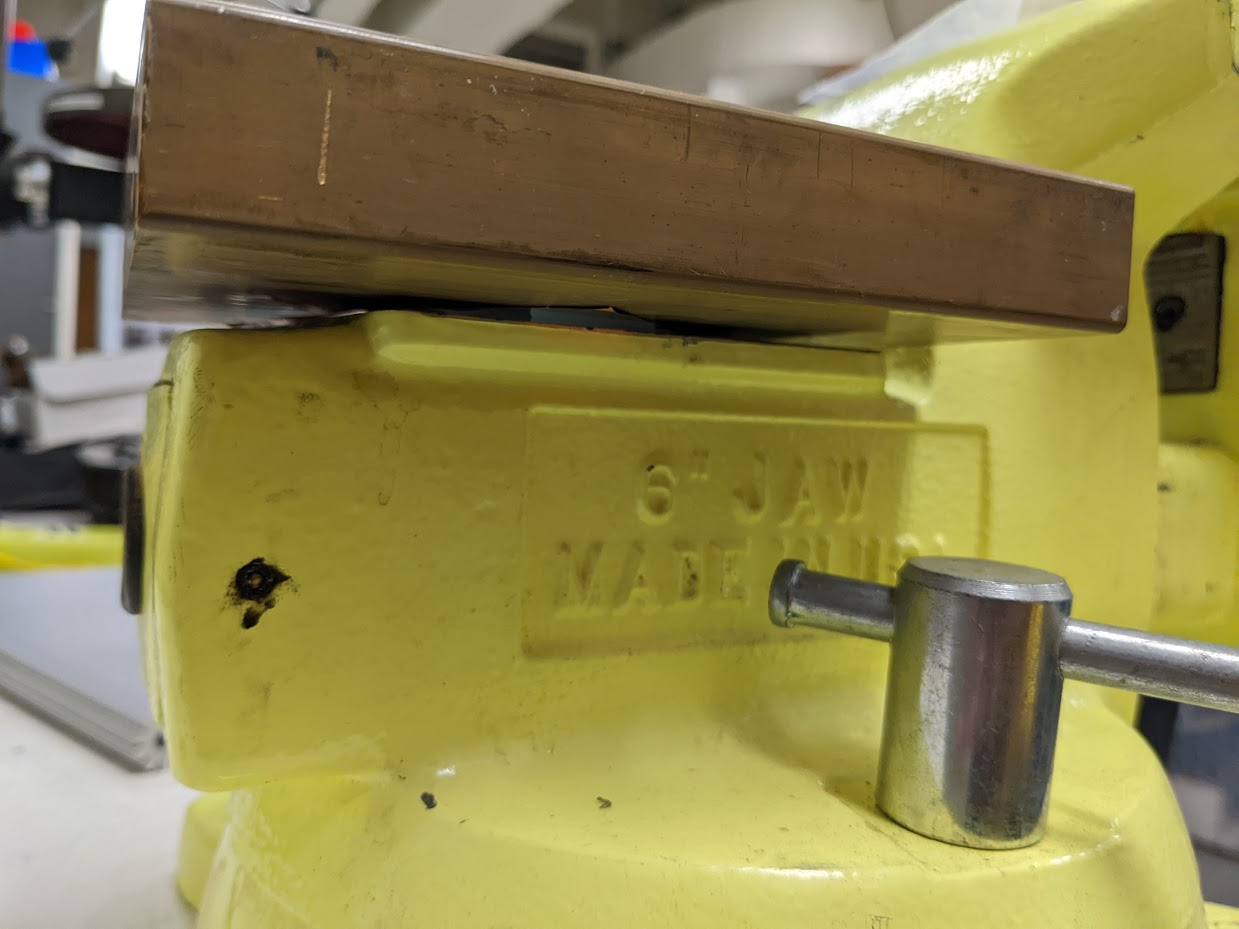
\includegraphics[width=6in]{graphics/squished_sample_PXL_20220712_025117243.jpg}
\caption{This is a bonded sample underneath the heavy brass mass. There is copper foil between the glass and metal to provide a buffer.}
\label{fig:squished_sample}
\end{center}
\end{figure}

Previous evidence suggested that heat would improve the strength of the bond. I tried heating the bonded samples many times, both without pressure {{{{fig}}}} and with a heavy brass mass on top of the sample {{{fig}}}. However, even a small amount of heat would almost immediately break even the strongest of bonds.

\begin{figure}[htbp]
\begin{center}
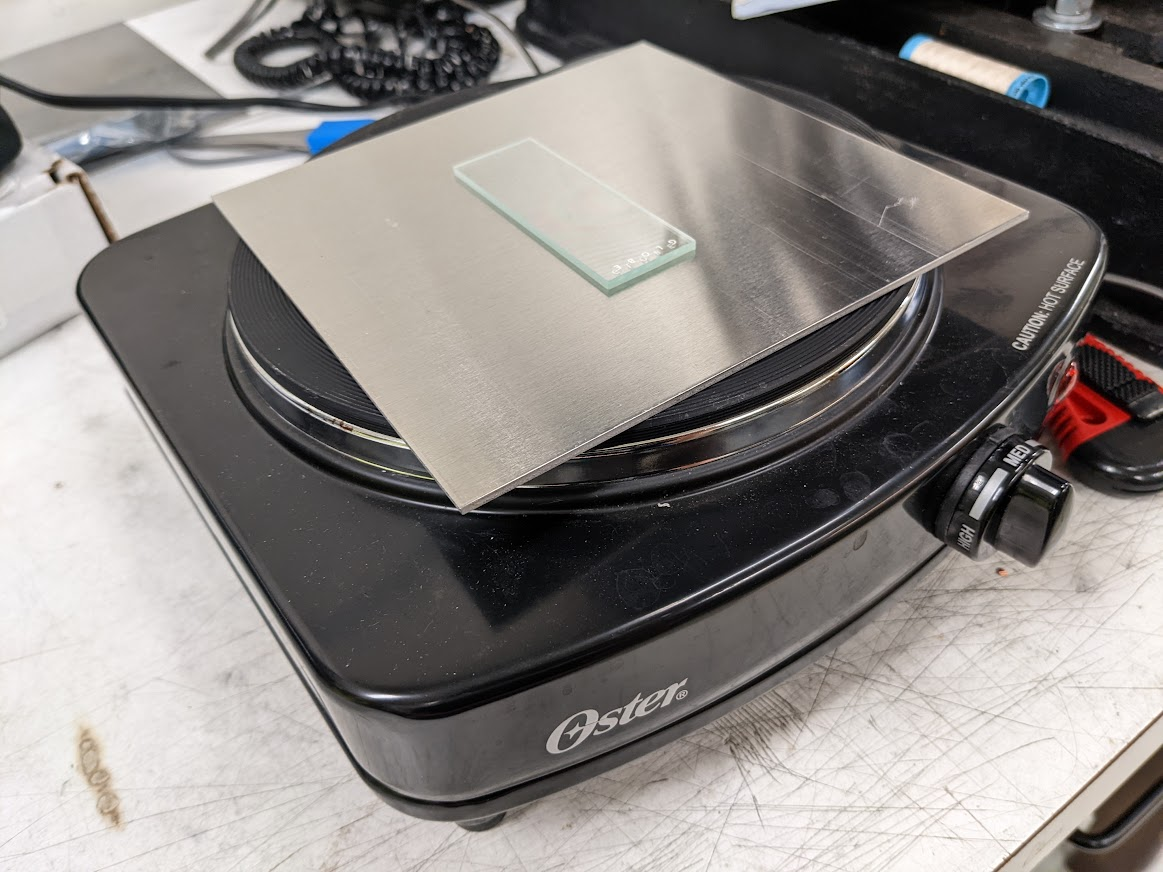
\includegraphics[width=6in]{graphics/heat_without_pressure_PXL_20220712_232551854.jpg}
\caption{To heat a sample without pressure, I simply place it on copper foil (not pictured) on the aluminum plate, which will have a thermocouple attached to it in the future, and turn on the heat. I will also sometimes preheat it.}
\label{fig:heat_without_pressure}
\end{center}
\end{figure}

\begin{figure}[htbp]
\begin{center}
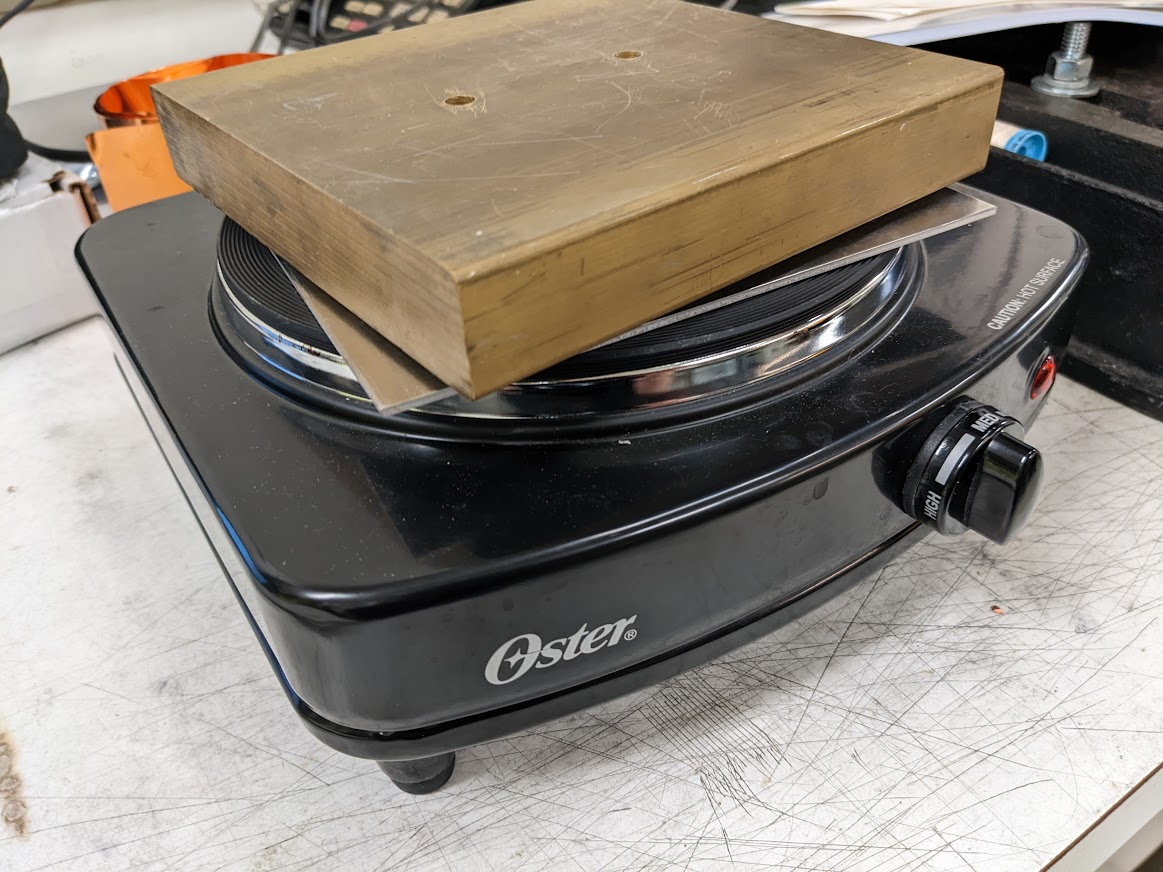
\includegraphics[width=6in]{graphics/heat_with_pressure_PXL_20220713_003923957.jpg}
\caption{To heat a sample with pressure, I do the same as without pressure, but with the brass weight on top and copper at the metal-glass interface. I cannot preheat this setup without risking burning my fingers.}
\label{fig:heat_with_pressure}
\end{center}
\end{figure}

Most recently, I have been trying to achieve a bond without the assistance of liquids, pressure, or heat. I have managed to produce a bond by scrubbing the slides with methanol, letting them dry, and then rubbing the two cleaned surfaces together while adding pressure. When I clean with methanol, I scrub with enough pressure to make them squeak. This bonding method is unreliable, and the bond is not as strong as when I use liquids.

\section{Progress}

As expected, while optical contacting seems simple on paper, actual bonding is quite difficult. I was still hoping to be a little further along by this point, but struggling with the heating conundrum and being absent from the lab slowed me down. Since I did not expect heating to break the bond, I was left a little directionless as I tried different bonding methods, mistakenly thinking that it was the method, not the heat, that was breaking the bond.

\section{Problems}

The biggest problem, as already mentioned in detail, is that the heat is unexpectedly breaking the bond instead of improving it. Although I have not identified the source of the problem, several theories have been proposed. My latest theory is that it is the rapidity of the heating that breaks the bond, but I have not been able to test it.

Another problem is that I should be able to achieve a bond without without liquid, pressure, or heat, but I have been unable to. If it is an issue of me not cleaning the glass well enough, I just need to improve my methods, like perhaps using First Contact Polymer or pressurized air during the cleaning process. If it is an issue of the glass not being polished enough, that could only be fixed by polishing the glass.

\section{Goals}

While writing this, I realized that I did not do a good job of systematically testing each method of glass bonding. I would like to spend a day or two systematically running through all the configurations of liquids (or therein lack of), heat, pressure, etc. so I have better, clearer data on what does and does not work. However, now that I have acquired silicon wafers, I would also like to start working with that as I am very curious to see if heat breaking the bond is an issue for silicon as well.

My current focus is further improving my bonding technique. If I do end up resolving the issue of heating breaking the bond, I will proceed as originally planned with creating a setup that lets me precisely control the temperature on the hot plate. Time is running short, so I am not sure if I will get to the bond quality experiments I had planned. It all depends on whether I am able to make a breakthrough on bond quality.

\begin{thebibliography}{9}
    \bibitem{Wright}
	  Wright, J. J. & Zissa,
	  \emph{D. E. OPTICAL CONTACTING FOR GRAVITY PROBE STAR TRACKER}.
	  14 (1984).    
      
    \bibitem{Rayleigh}
	  Rayleigh, Lord,
	  \emph{Optical Contact}.
	  Nature 139, 781–783 (1937).
	  
	\bibitem{Ferme}
	  Ferme, J.-J.,
	  \emph{Optical contacting}.
	  in (eds. Geyl, R., Rimmer, D. & Wang, L.) 26 (2004).
	 
    \bibitem{Zawada}
	  Zawada, A.,
	  \emph{Final Report: In-Vacuum Heat Switch}.
	  14.
    
	\bibitem{Helie}
	  Hélie, David, et al.,
	  \emph{Reinforced direct bonding of optical materials by femtosecond laser welding}.
	  Applied optics 51.12 p.2098-2106 (2012).    

	\bibitem{Ohlidal}
	  He, Mengfei, and Sidney R. Nagel,
	  \emph{Ellipsometry of layered systems}.
	  Optical Characterization of Thin Solid Films. Springer, Cham, p.233-267 (2018).

	\bibitem{Kurz}
	  Kurz, Volker Luiz Siegmar.,
	  \emph{Orientation, conformation and phase transitions of thin polymer films and self-assembled monolayers studied by SFG spectroscopy}.
	  Diss. (2010).

    \bibitem{Zawada2}
	  Zawada, A.,
	  \emph{Determining the refractive index, absolute thickness and local slope of a thin transparent film using multi-wavelength and multi-incident-angle interference}.
	  Optics Express 28.16 p.24198-24213 (2020).
  
    \bibitem{Kalkowski}
	  Kalkowski, Gerhard, et al.,
	  \emph{Glass-glass direct bonding}.
	  ECS Transactions 64.5 p.3 (2014).
 
\end{thebibliography} %Must end the environment

\begin{appendices}

\section{Bold quality experiment drafts}
\label{appendix:bond_quality_experiment_drafts}
\subsection{Shear strength}
\subsubsection{First design}

My design was inspired by the apparatus used in a paper which was measuring the shear strength of a glass-glass direct bond \cite{Helie}. The paper had a picture of their apparatus (Figure \ref{fig:apparatus}) but did not explain how their apparatus was constructed---most importantly, they did not explain how they mounted their wafers---so I had to design that myself.

\begin{figure}[htbp]
\begin{center}
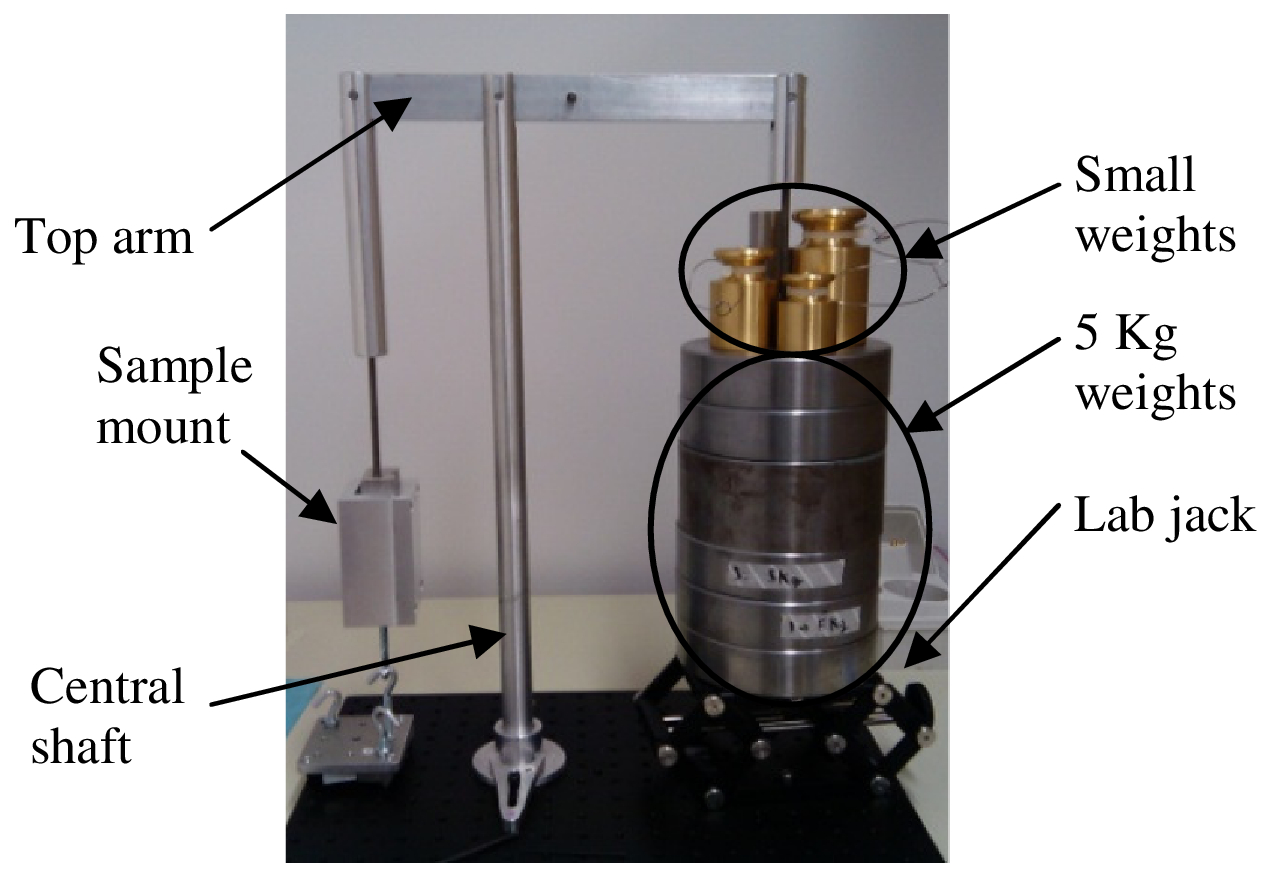
\includegraphics[width=6in]{graphics/apparatus.png}
\caption{"Photograph of the setup used for shear strength measurements." \cite{Helie}.}
\label{fig:apparatus}
\end{center}
\end{figure}

The shear strength is measured by mounting the optically bonded wafers on one side of a beam balance then slowly adding weight to the other side until the bond is broken. As shown in Figure \ref{fig:myapparatus}, the bonded wafers are mounted such that weight pulls up one side while the other remains secure. A lab jack is used to assist with adding the weights.

\newpage

\begin{figure}[htbp]
\begin{center}
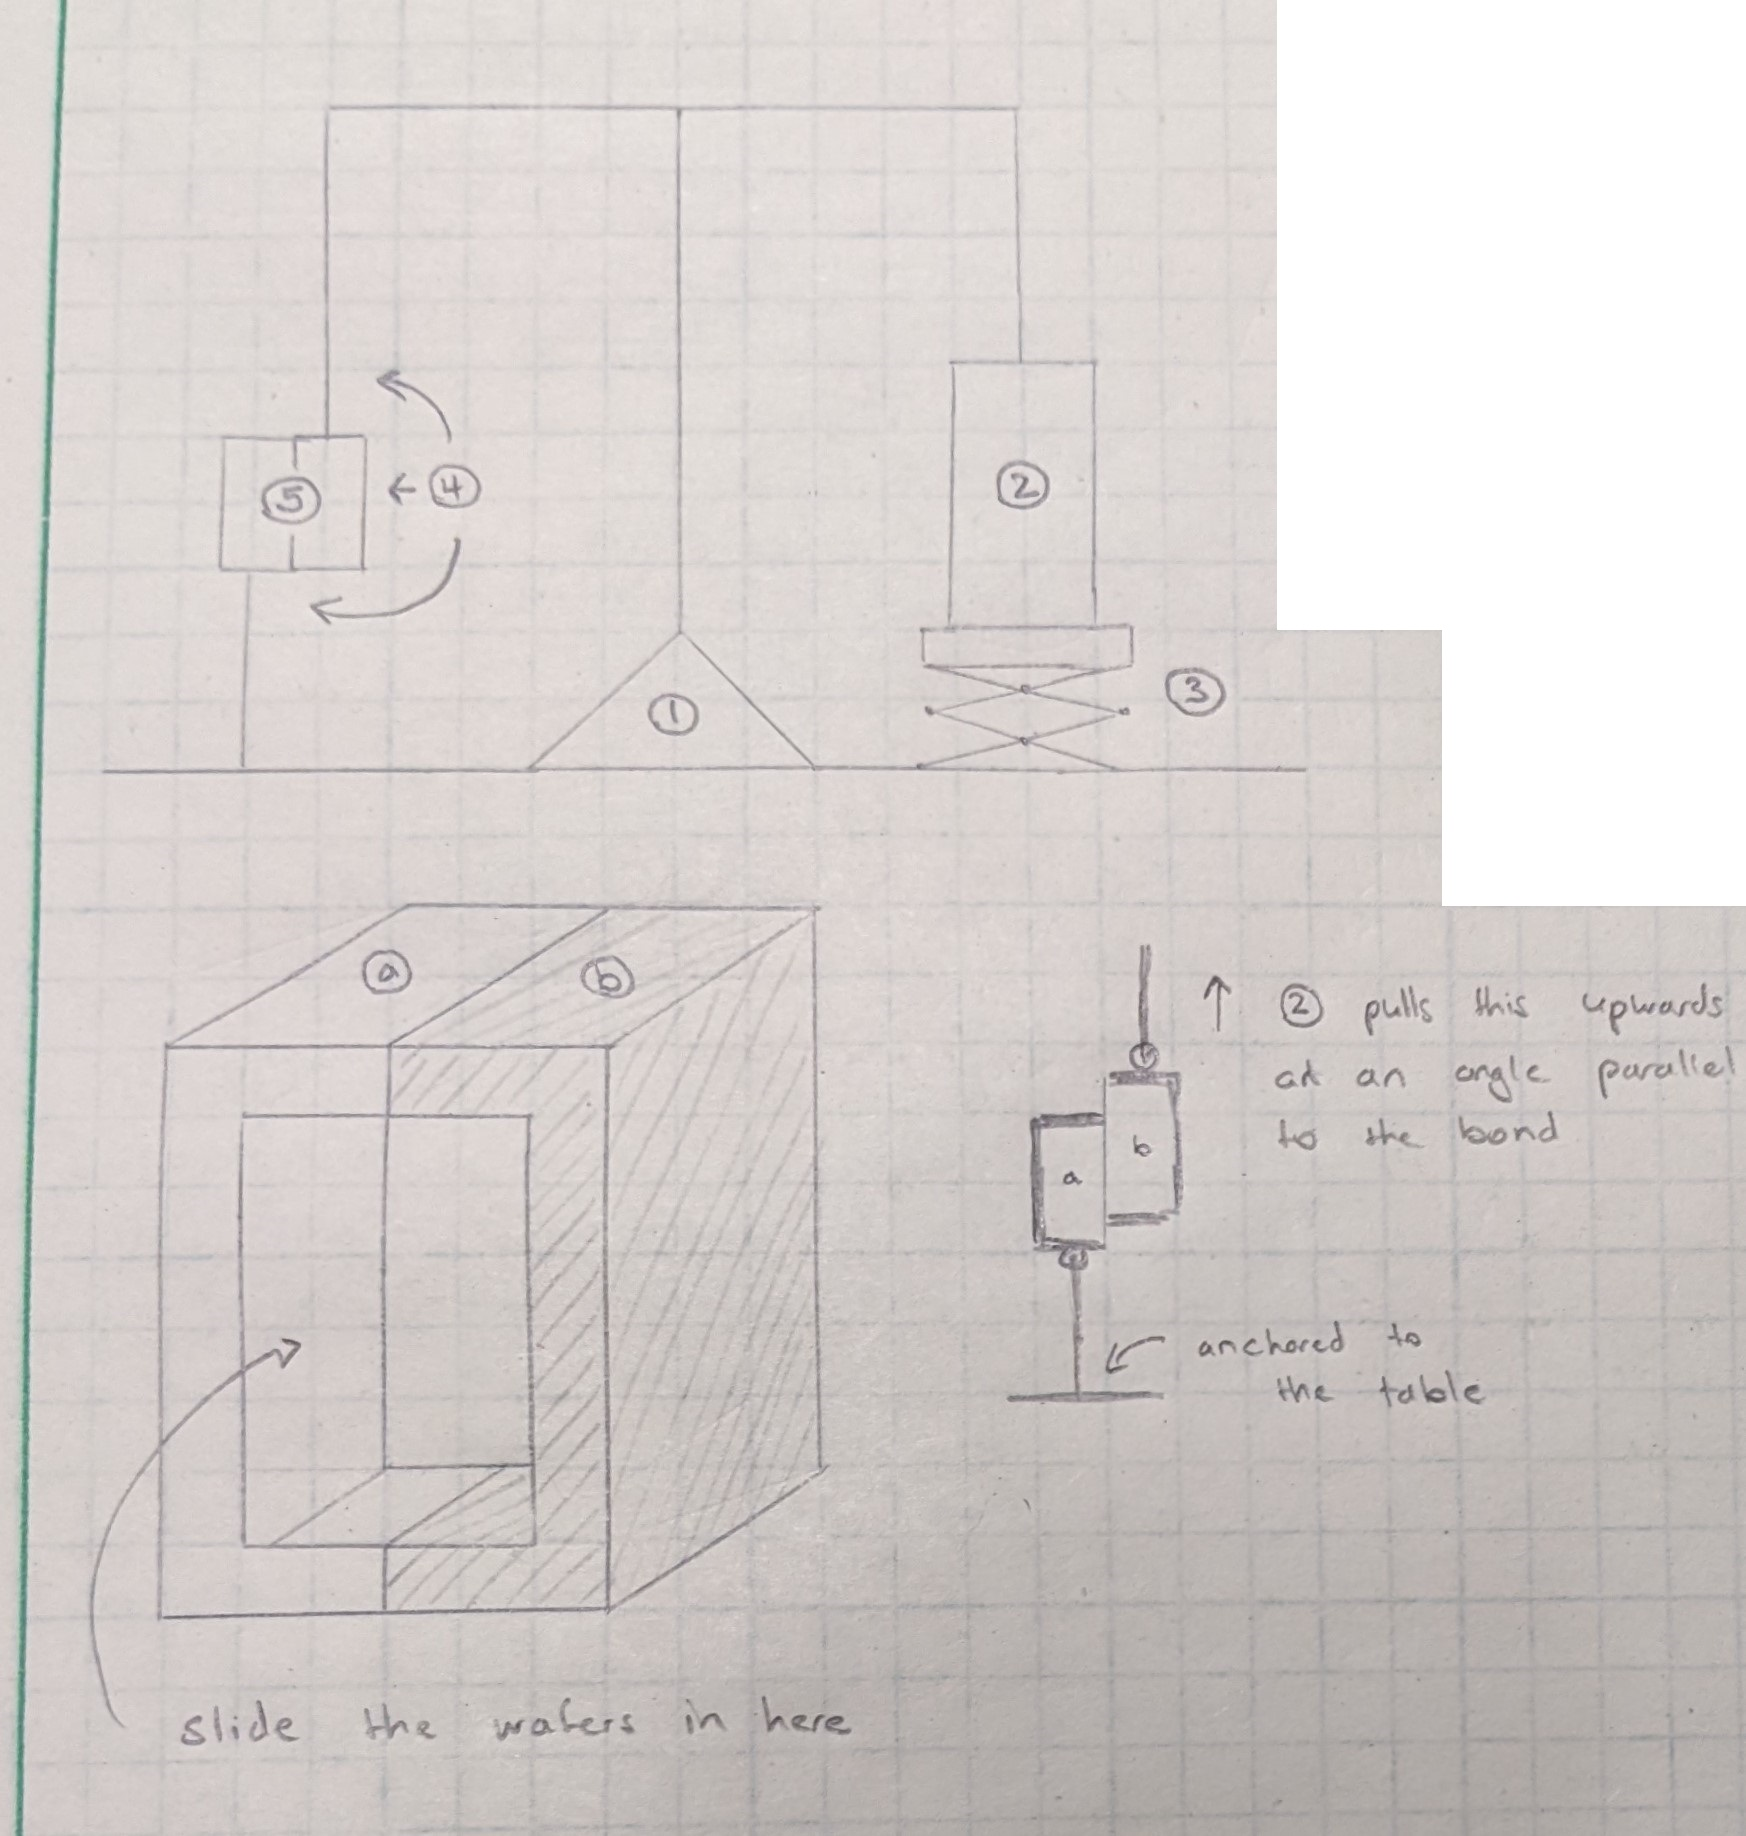
\includegraphics[width=6in]{graphics/scratchwork.jpg}
\caption{My design of my apparatus and the mount for the bonded wafers as well as a crude diagram of how the apparatus functions.}
\label{fig:myapparatus}
\end{center}
\end{figure}

\newpage

Parts list:

\begin{enumerate}
  \item Traditional beam balance
    \begin{itemize}
    \item I am not sure if this can be purchased or it will need to be constructed. It seems simple enough to me, but I could be underestimating its complexity.
    \item If it needs to be constructed, I can put together a list of the parts needed.
    \end{itemize}
  \item Various weights (total to roughly 100 kg)
    \begin{itemize}
    \item The idea is to slowly add smaller weights until you reach a certain amount then remove them and add a big single weight equivalent to their weight. Repeat until failure.
    \item I swear I have seen weights like in Figure \ref{fig:apparatus} used in a lab class, so I presume they are not something that needs to be purchased.
    \end{itemize}
  \item Lab jack
    \begin{itemize}
    \item This is for taking the weight off the bonded wafers while replacing the smaller weights with the big single weight.
    \end{itemize}
  \item Mount for bonded wafers
    \begin{itemize}
    \item This was the hardest part to design since it needs to be a snug fit while also being capable of bearing weight. My idea is to 3D print a casing like in Figure \ref{fig:myapparatus}. I am unsure if I can 3D print with a material strong enough to bear the weight, so perhaps metal should be attached around them. The mount is attached to the beam balance with a hook.
    \end{itemize}
  \item Bonded wafers
    \begin{itemize}
    \item These will be on the OOM of 10mm x 10m x 1mm. If it is cheaper/quicker to get a slightly different thickness (0.5mm looked more common based on a quick Internet search), that will work as well.
    \item It has to be fairly small otherwise it will be infeasible to add enough weight to break the bonds. The inspirational paper used similar OOM glass wafers and reported 75kg being the max it took to break them.
    \end{itemize}
\end{enumerate}

\subsubsection{Complications}

In practice, my first design would probably not work, especially for silicon which is extremely thin and fragile. Instead of finding the shear strength, I may have to replace this measure with finding the tensile strength.

\subsection{Index of refraction}

Finding the absolute thickness of a thin film requires a technique known as ellipsometry. Basic ellipsometry is shown in Figure \ref{fig:PCSAellipsometer}. It works on the principal that the polarization of incident light changes upon reflection against a sample \cite{Ohlidal}. Since I am working with multiple layers, my set up will look more like Figure \ref{fig:myellipsometer}.

\begin{figure}[htbp]
\begin{center}
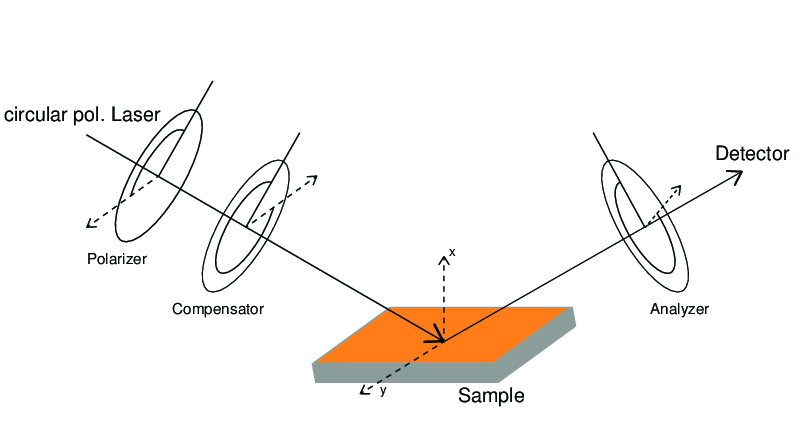
\includegraphics[width=6in]{graphics/Ellipsometer-in-a-PCSA-configuration.png}
\caption{PCSA ellipsometer in reflection mode \cite{Kurz}.}
\label{fig:PCSAellipsometer}
\end{center}
\end{figure}

\begin{figure}[htbp]
\begin{center}
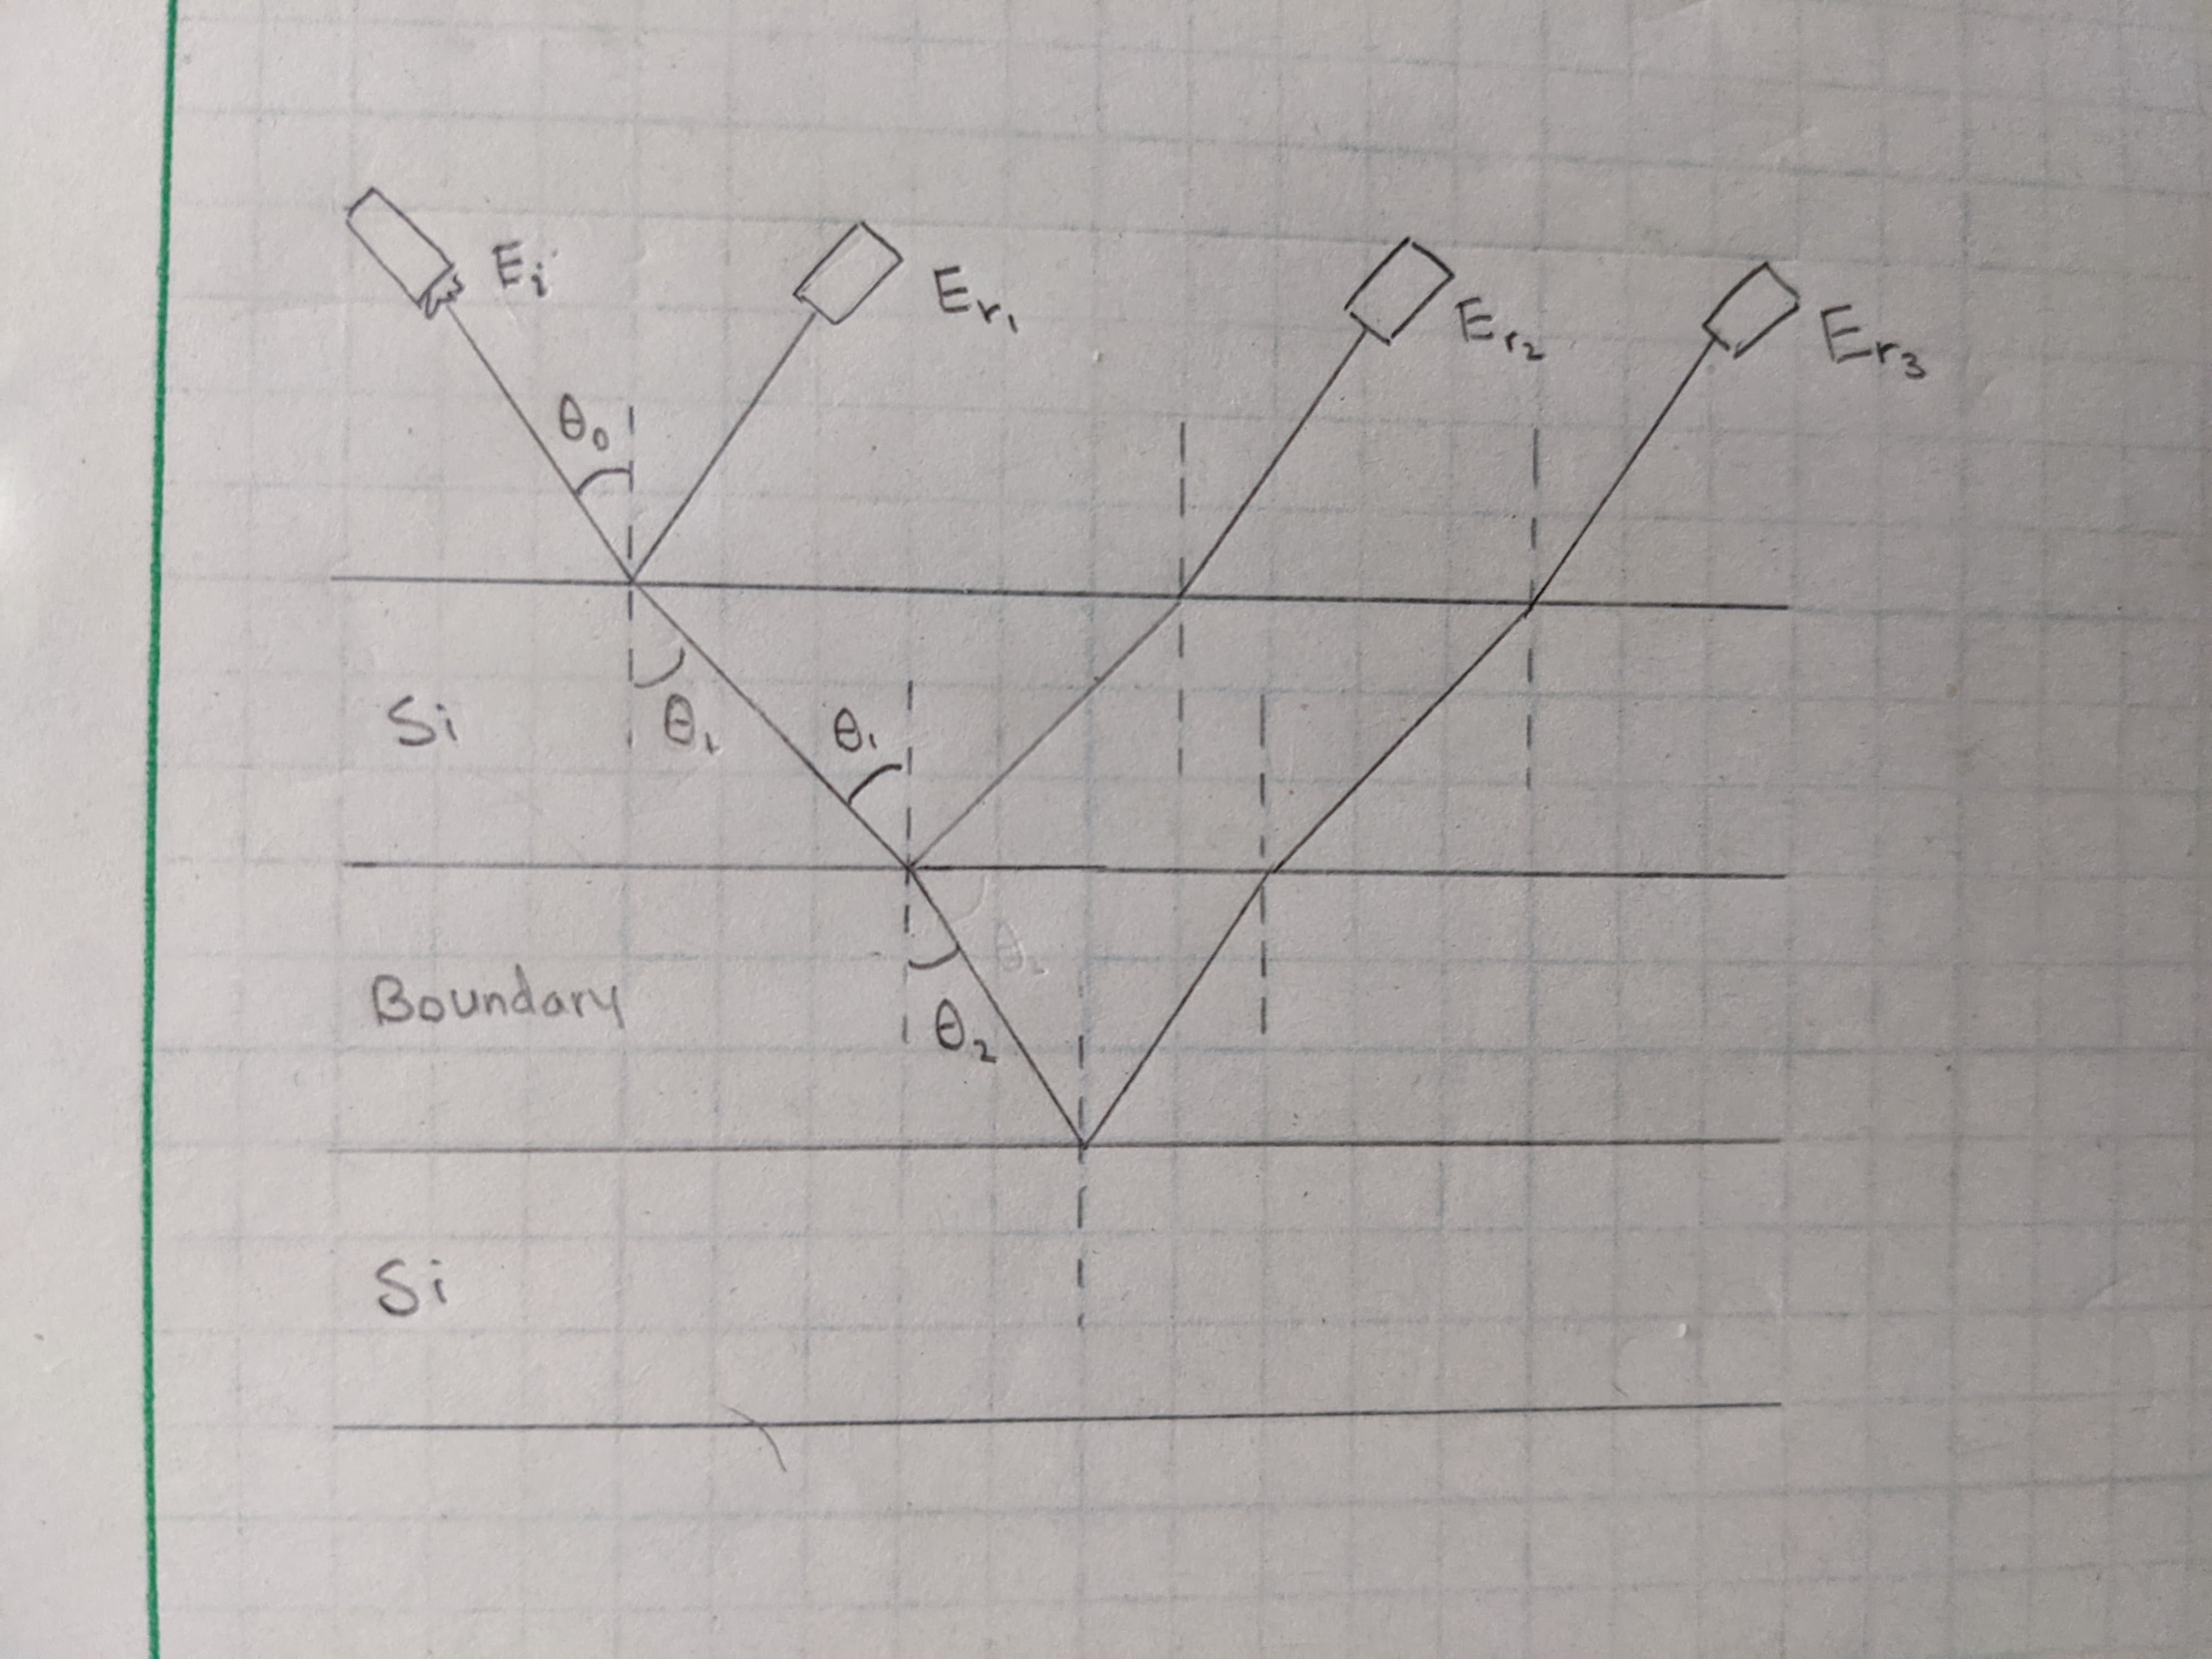
\includegraphics[width=6in]{graphics/my_ellipsometry.jpg}
\caption{Adapting figure \ref{fig:PCSAellipsometer} for multiple layers. Optical pieces like the polarizer and compensator are not shown.}
\label{fig:myellipsometer}
\end{center}
\end{figure}

\newpage

Basic parts list:

\begin{enumerate}
    \item Laser source
        \begin{itemize}
        \item It will be 1550 nm.
        \item I may be able to replace it with an IR LED.
        \end{itemize}
    \item Linear polarizer
    \item Compensator (optional?)
        \begin{itemize}
        \item "Introduces a defined phase retardation of one field component with respect to the orthogonal field component, the sample S, the analyzer A, and a detector" \cite{Kurz}.
        \item I am a bit confused on what this part does, to be frank. It appears to be optional for reasons that I do not understand.
        \end{itemize}
    \item Sample
        \begin{itemize}
        \item I believe I will be able to use the same size wafers as the shear strength experiment. As I will elucidate after this list, I have been struggling with doing the exact math, so this is just based on reading a several papers which used OOM 10mm x 10m x 1mm thin films.
        \end{itemize}
    \item Detector
\end{enumerate}

Actually putting this technique into practice is not straightforward---at least for someone like me who does not have an abundance of experience with experimental optics, although based on the papers I read, this does appear to be a difficult problem in general. The math is all linear algebra, but due to the number of variables, actually doing the calculations is quite overwhelming, especially when I am struggling to understand what is happening conceptually. There are also limits to capabilities of ellipsometry, as the changes in index of refraction may be so small that they are virtually undetectable \cite{Kalkowski}. The diagram in Figure \ref{fig:PCSAellipsometer} is also considered the simplest case; due to the complexity of my specific experiment, I may need to use a more complicated form of ellipsometry.

\subsection{Mechanical q}

I began writing code to find the best dimensions of the silicon tuning fork for maximum precision and accuracy, but some of the variables that I thought were constant turned out to not only be variable in ways that could not be predicted by equations. Before I could figure out how to interpolate the real world variable data, I had to turn my focus to other parts of the project.

\end{appendices}

\end{document} 